\begin{frame}
  \frametitle{Plan du cours}
\tableofcontents

\end{frame}

\begin{frame}
  \frametitle{Le Clustering une discipline de Machine learning}

 \begin{figure}
  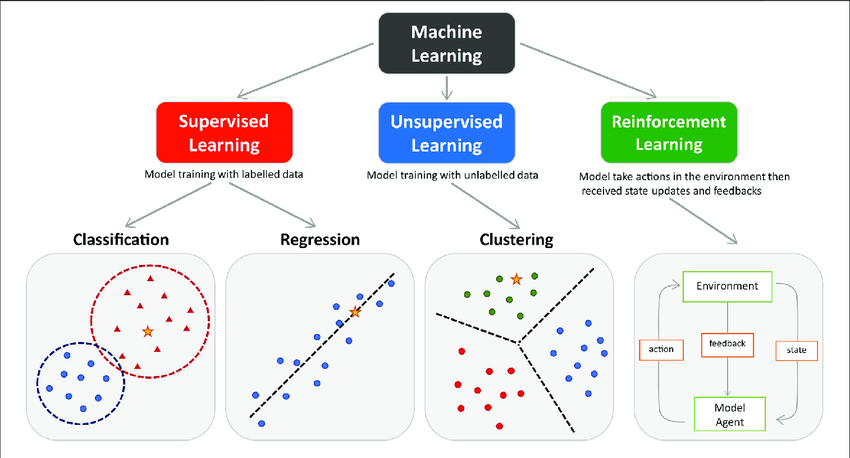
\includegraphics[width=10cm]{images/The-main-types-of-machine-learning-Main-approaches-include-classification-and.png}
  \caption{\url{https://www.frontiersin.org/journals/pharmacology/articles/10.3389/fphar.2021.720694/full}, \cite{10.3389/fphar.2021.720694}}
  \end{figure}
\end{frame}

\begin{frame}
  \frametitle{Définition }


\end{frame}

\begin{frame}
  \frametitle{Le clustering en TAL}


\end{frame}

\begin{frame}
  \frametitle{Le clustering en TAL : à quoi ça sert ?}
  
  \begin{itemize}
  \item Regrouper des textes
  \item Regrouper des mots 
  \end{itemize}


\end{frame}

\begin{frame}
  \frametitle{Le clustering en TAL : quelles méthodes}

  \begin{itemize}
  \item Hiérarchique dendogrames
  \item Centroïde K-mean, Affinity Propagation
  \item A densité
  \end{itemize}
  
\end{frame}

\begin{frame}
  \frametitle{Hiérarchique dendogrames}

  
\end{frame}

\begin{frame}
  \frametitle{Centroïde}


  
\end{frame}

\begin{frame}
  \frametitle{A densité}


  
\end{frame}
